\documentclass[a4paper,conference]{IEEEtran}
\IEEEoverridecommandlockouts
% ============ PACKAGES =============

% *** CITATION PACKAGES ***
\usepackage{cite}
% *** COMMON MATH PACKAGES ***
\usepackage{amsmath,amssymb,amsfonts}
% *** GRAPHICS RELATED PACKAGES ***
\usepackage{graphicx}
% *** TABLES RELATED PACKAGES ***
\usepackage{booktabs}
% *** PDF, URL AND HYPERLINK PACKAGES ***
\usepackage{url}
% *** SPECIALIZED LIST PACKAGES ***
\usepackage{algorithmic}
% *** SUBFIGURE PACKAGES (MANDATORY) ***
\usepackage{subcaption}
\captionsetup[figure]{name={Figure},labelsep=period, font=footnotesize}
\captionsetup[table]{labelsep=period, font={sc,footnotesize} }

% ============ COMMANDS =============

\newcommand{\authorfont}{\fontsize{11pt}{10pt}\selectfont}
\renewcommand\IEEEkeywordsname{Keywords}

% some macros for maths
\newcommand{\bs}[1]{\boldsymbol{#1}}
\newcommand{\ma}[1]{\bs{\mathcal{#1}}}
\newcommand{\seq}[1]{\bs{#1}}
\newcommand{\set}[1]{\mathcal{#1}}

% ============ DOCUMENT STARTS HERE ============ 

\begin{document}

\title{Prototyping Cellular Command-and-Control Platform for UAS \\\vspace{10pt} }

\author{\IEEEauthorblockN{\authorfont Boris Resnick}
\IEEEauthorblockA{\normalsize Chief Technology Officer \\
\normalsize Flyvercity \\
\normalsize Netanya, Israel \\
\normalsize boris@flyver.city}
}

\maketitle

\begin{abstract}
The paper describes a basic architecture and implemementation details of a edge-native platform for command-and-control of Unmanned Aviation Systems (UAS) via a cellular network. Discovery, reliability, security, and decentralized authorization aspects are discuss.
\end{abstract}

\begin{IEEEkeywords}
UAS, drones, cellular, C2, 5G, MEC
\end{IEEEkeywords}

\section{Introduction}
Over the coming years, the use of Unmanned Aviation Systems (UAS) a.k.a. drones will expand massively. Urban skies will become more and more packed with UAS. The number of flights and associated safety risks would increase accordingly.

A new world of product and service delivery will emerge. Most of these operations would be conducted in beyond visual line of sight (BVLOS) mode, and therefore aviation-grade reliable command-and-control link would be required. Without this critical part scaling of the industry is impossible, and therefore the global potential of air mobility market (once estimated as \$1.5 trillion \cite{market}) will remain unrealized. 

When UAS command-and-control (C2) connectivity employs a cellular network, specifically for BVLOS, there is a number of considerations for an operator to resolve. These issues are driven by required capabilities, standardization, and regulation.

While an operator may able to implement all C2 aspects by themself, scalability requirements call for a more centralized and coordinatied approach. This is where a C2 middleware platform comes into play. Our general approach to address this problem is defined the this paper \cite{uai}.

We identify the following aspects of C2 connectivity that need to be addressed:

\begin{itemize}
\item establish a discovery mechanism between airborne and ground entities.
\item manage reliability of connection by interacting with 5G network functions.
\item support data transmission security by managing security credentials as defined by aviation regulation \cite{icao:annex10VI} and \cite{rtca:do377a}.
\item support aerial connection authorization to address emerging regulatory requirements as defined by telecom regulation \ref{3gpp:uual}
\item monitor performance and compliance by signal data acquisition and analysis.
\item manage remote pilot station (RPS) access to drones under control.
\end{itemize}


\section{Commmand-and-Control Middleware Platform}

This paper describes a possible approach to address the above issues. The approach is based on the following principles:

\begin{itemize}
\item The platform is based on a cloud native architecture.
\item The platform is designed to be deployed on mobile network operator's (MNO) resources, following the concept of multi-acceess edge computing (MEC).
\item The implementation in open-source and extensible.
\end{itemize}

There are two types of users of the platform:

Aerial Connection Users are flying objects equipped with 5G user equipment (UE) and requiring to establish a reliable connection. Generally these are Aerial Vehicles a.k.a. drones. These also may include Wireless RPS a.k.a. ground control stations (GCS).

Aviation Data Exchange (ADX) Users are stationary entities that connect to aerial users via the ADX, but not via any 5G radio. These are generally fixed ground control center workstations.

\subsection{Discovery and Connections}

The main use case of the service is the Session Establishment procedure reflected on the following diagram:

\begin{figure}[!ht]
\centering
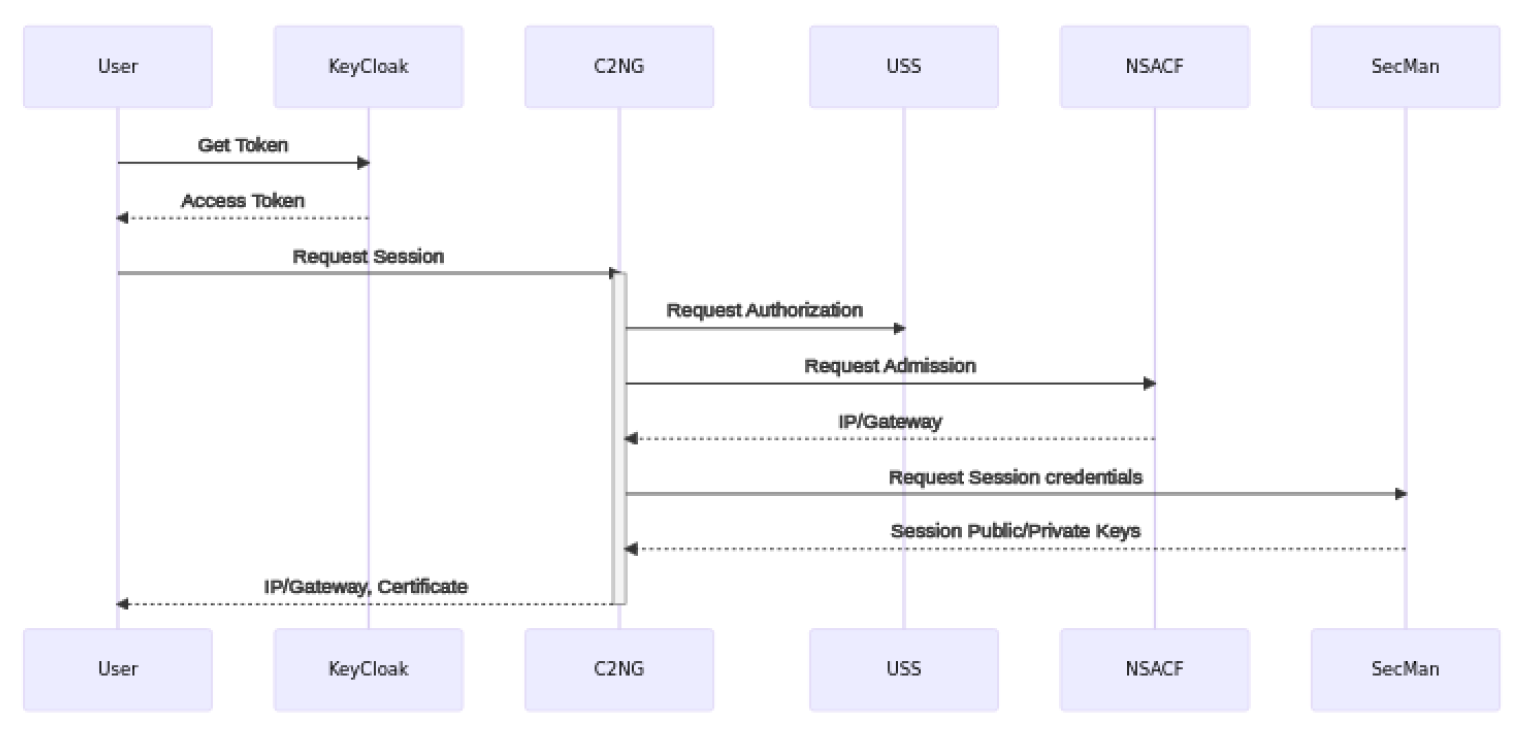
\includegraphics[width=0.9\linewidth]{images/session.png}
\caption{Session Establishment Procedure}\label{fig:session}
\end{figure}

A central concept used by the service to enable discovery procedures is Logical ID. The same uncrewed vehicle may represented by different identification schemas, include civil aviation authority-issued identification number, internal ID of a drone operator, a designator used by Uncrewed Traffic Management (UTM) system, or 3GPP-defined identifier such as IMSI (International Mobile Subscriber Identity). The service maintains the mapping between all these identification schemas to a single Logical ID. The Logical ID is used to identify the drone, as well as the RPS, in all interactions with the service. This enables a transparent discovery procedure, where the service is able to identify the drone and its RPS, regardless of the identification schema used by the drone operator.

Main flow on the connection procedure supported by the service is as follows:

\begin{enumerate}
\item The drone requests a connection session by providing the Logical ID of the drone and the RPS.
\item The service performs lookup of the relevant drone and RPS identifiers by the Logical IDs.
\item The service creates a connection session.
\item Network management subsystem select a proper MNO and ADX, and ensures that network quality of service configuration is relevant to the session requirements.
\item The service request an authorization from the relevant UTM system and supports the authorization procedure, which will be initiated by the 5G network \ref{reliability}.
\item The service creates session security credentials (\ref{security}) and provides them to the drone and the RPS together with the connection parameters.
\end{enumerate}

This procedure enables truly dynamic discovery and connection procedures, where the drone operator is not required to pre-register the drone with the RPS and vice versa. The service is able to identify the drone and the RPS by the Logical ID, and the drone operator is able to use any identification schema they prefer.

\subsection{Reliability}

The primary goal of the service is to ensure reliable connectivity between the drone and the RPS. The service is able to achieve this goal by interacting with the 5G network functions. First of all, the service is able to request a specific network slice to be allocated to the session. The service is also able to request a specific quality of service (QoS) configuration.

For the perspective of the requested drone operation, the QoS is determined by the following parameters (RLP - Required Link Performance as defined by \cite{rtca:do377a}).

{\b Availability} is minimum percentage of time that the services of the system are usable with the level of guarantee on latency and throughput.

{\b Continuity} is an acceptable probability message is delivered successfully after its transmission was started assuming the communications system is available when the transmission is initiated. Any error that can be corrected on a transport level or below is not included here.

{\b Integrity} is an acceptable probability of elementary message transmission was completed with an undetected error. Error is detected if sending party receives a timely (within latency time) notification from Data Transmission Service. Loss of integrity includes a risk of data corruption due to tampering and other possible security issues.

An external user, such as a drone operator, is not able to determine a mapping between these parameters and network configuration. On the contrary, the service, being tighly integrated with the network, can derive feasibility of QoS provision and necessary measures.

Parameters controlled by the network may vary depending on the given network architecture. During our trials, we used two-step procedure:

\begin{enumerate}
\item RLP parameters looked up in the database based on the drone type and the requested operation.
\item Based on Availability/Continuity failure, the service selected one of a set pre-configured network slices.
\item The slice's 5QI (5G QoS Identifier) was adjusted based on latency requirement.
\item Overall throughput analysed to avoid any overloads.
\item New user (aerial or an ADX) was added to the slice via the NSACF.
\end{enumerate}

It also worth mentioning that these technical provisions should be supported by organizational means such as SLA (Service Level Agreements) when deployed operationally.

\subsection{Security}

tbd

\subsection{Aerial Connection Authorization}

tbd

\subsection{Performance Monitoring}

tbd

\subsection{Remote Pilot Station Access}

To help drone operators (designate this section as "owners") to manage their fleet, the platform provides a mechanism to manage access to the drones by remote pilot stations (RPS).

\begin{figure}[!ht]
\centering
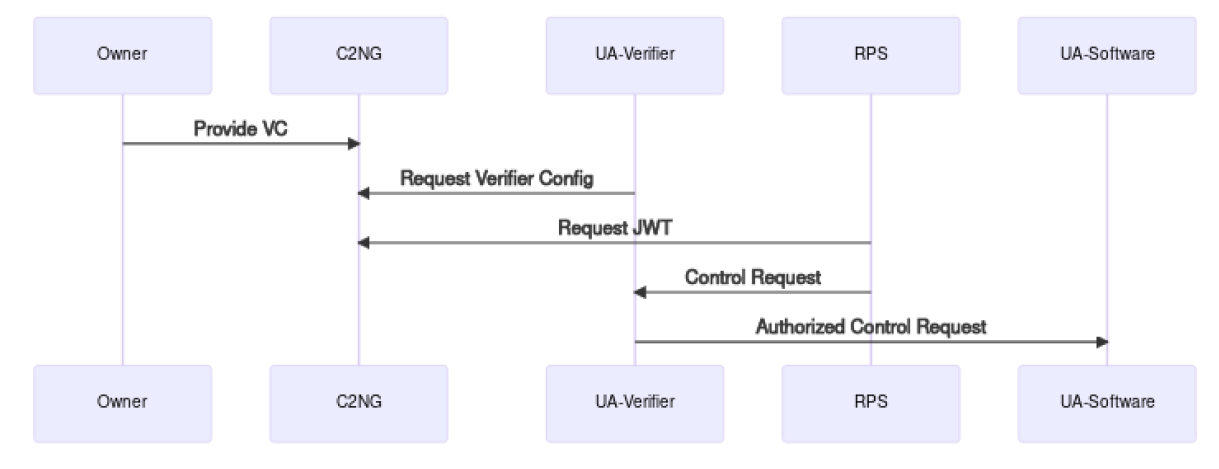
\includegraphics[width=0.9\linewidth]{images/did.png}
\caption{Decentralized Identification}\label{fig:did}
\end{figure}

The platform supports remote pilot station authorization to control the drones via the advanced decentralized identification mechanism \cite{excid:did}. The DID solution provides the Verified Credentials mechanism which allows the platform or its users to manage authorization without permanent connection to the drones or the pilot stations themselves.

The platform supports the following "key" and "self" DID types, and can serve as a drone owner or support drone operator as an owner. For purposes of the decentralized authentication mechanism, the owner is a entity that issues a Verifiable Credential to their RPS station under control.

A drone itself implemement a verifier that operates based on the verifier configuration provided by the platform. The verifier is able to determine if the RPS is authorized to control the drone, based on the encrypted token provided by the RPS.

% \begin{table}[ht!]
%   \begin{center}
%     \caption{Example of generic table}
%     \label{tab:table1}
%     \begin{tabular}{@{}lcr@{}} % <-- Alignments: 1st column left, 2nd middle and 3rd right
%       Column 1 & Column 2 & Column 3 \\
%       $\alpha$ & $\beta$ & $\gamma$ \\
%       \hline
%       1 & 1110.1 & a\\
%       2 & 10.1 & b\\
%       3 & 23.113231 & c\\
%     \end{tabular}
%   \end{center}
% \end{table}

\section{Implementation and Evaluation}

\subsection{Application Architecture}

The Application is based on containerized services and comprises three open source basic components (KeyCloak, MongoDB, and InfluxDB) and the core software service (C2NG). Besides the core software, CLI (command line interface) tools was developed to control all administrative task, simulation and demostration. KeyCloak is an open source implementation OIDC (Open ID Direct Connect) protocol and supports authorized calls to the service.

\begin{figure}[!ht]
\centering
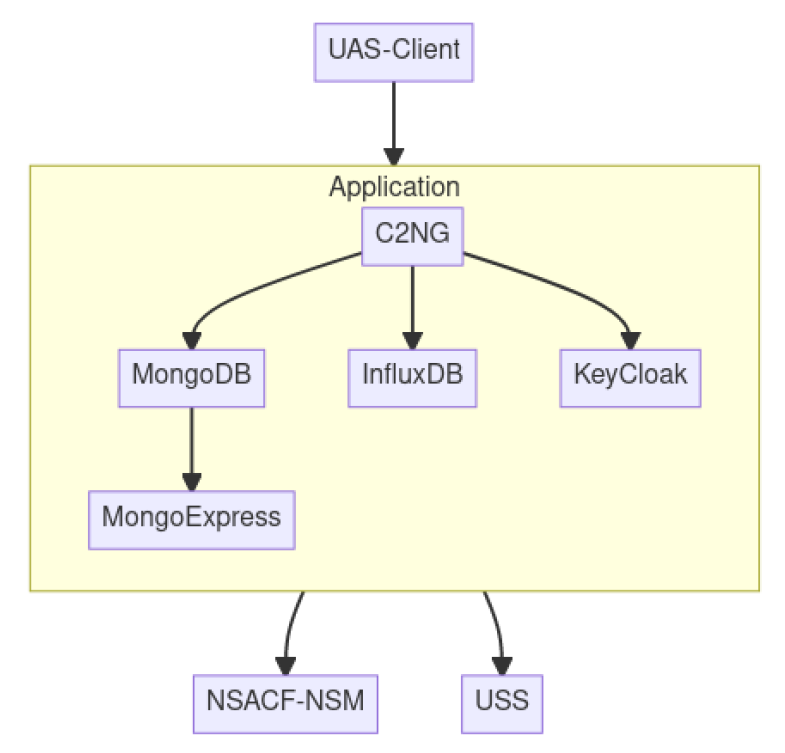
\includegraphics[width=0.9\linewidth]{images/arch.png}
\caption{Decentralized Identification}\label{fig:arch}
\end{figure}

NSACF (Network Slice Admission Control Function) is a Network Function exposed by the 5G Core to control which users are authorized to use a slice, and hence enjoy high-reliablity allocated to it. It can be also extended by a particular implementation to control 5G slices in a more fine-grained manner (the umbrella term for this is “Network Slice Management” --- NSM).

MongoDB is a NoSQL database that serves as a persistence layer. The database is schema-less, but a logic schema is described is the corresponding section. InfluxDB is a timeseries database used to collect signal characteristics reported by aerial users. C2NG designates the service itself. C2NG is a web service and exposes two APIs. The REST API described in the API Definition section is used by the users to request connectivity sessions and report signal quality information. The second API is is any web-socket based asynchronious API used to notify the users about the changes in the session status in real time.

The whole application is a set of Docker containers defined by the Docker Compose Specification for developement and single-node environments.

\subsection{Validation}

Network integration and quality-of-service subsystem was tested in the lab, associated with IoT-NGIN project, with an advanced 5G core is capable of managing the network slices and providing the required connectivity for the drones.

\section{Conclusion}
The conclusion goes here.

\section*{Acknowledgment}

This paper is based on the results of IoT UAS C2 project, a sub-project funded via the IoT-NGIN project Open Call. IoT-NGIN has received funding from the European Union’s Horizon 2020 research and innovation programme (Grant Agreement No 957246).

% can use a bibliography generated by BibTeX as a .bbl file
% BibTeX documentation can be easily obtained at:
% http://www.ctan.org/tex-archive/biblio/bibtex/contrib/doc/
% The IEEEtran BibTeX style support page is at:
% http://www.michaelshell.org/tex/ieeetran/bibtex/
%\bibliographystyle{IEEEtran}
% argument is your BibTeX string definitions and bibliography database(s)
%\bibliography{IEEEabrv,../bib/paper}
%
% <OR> manually copy in the resultant .bbl file
% set second argument of \begin to the number of references
% (used to reserve space for the reference number labels box)
\begin{thebibliography}{1}

\bibitem{IEEEhowto:kopka}
H.~Kopka and P.~W. Daly, \emph{A Guide to \LaTeX}, 3rd~ed.\hskip 1em plus
  0.5em minus 0.4em\relax Harlow, England: Addison-Wesley, 1999.

\end{thebibliography}
\end{document}